\documentclass[a4paper]{article}

% Packages
\usepackage{amsmath} % For math symbols and equations
\usepackage{amssymb} % For math symbols
\usepackage{enumerate} % For custom numbering of lists
\usepackage[
  inner=2cm, % Set inner margin to 2 cm
  outer=2cm, % Set outer margin to 2 cm
  bindingoffset=0.5cm, % Set binding offset to 0.5 cm
  top=2cm, % Set top margin to 2 cm
  bottom=2cm % Set bottom margin to 2 cm
]{geometry}
\usepackage{fancyhdr} % For custom headers and footers
\usepackage{lastpage} % For referencing the last page number
\usepackage{titlesec} % For custom section and subsection headings
\usepackage[version=4]{mhchem} % Required package for chemical equations
\usepackage{hyperref}
\usepackage[
backend=biber,
sorting=anyvt,
style = nature
]{biblatex} % for using references
\usepackage{parskip}
\usepackage{setspace}
\usepackage{graphicx}
\usepackage{cancel}
\usepackage{todonotes}
\setuptodonotes{inline}
\usepackage{caption}
\usepackage{adjustbox}
\usepackage{booktabs}
\usepackage[shortlabels]{enumitem}
\addbibresource{hw2refs.bib}

% Page setup
\pagestyle{fancy} % Set page style to fancy
\fancyhf{} % Clear default headers and footers
\lhead{Bekir Şahin} % Set left header to your name
\rhead{ENVE422 - Homework 2} % Set right header to assignment name
\rfoot{Page \thepage\ of \pageref{LastPage}} % Set footer to page number

% Section and subsection setup
\titleformat{\section}{\large\bfseries}{Question \thesection}{1em}{} % Set section format
\titleformat{\subsection}{\bfseries}{Part \thesubsection}{1em}{} % Set subsection format
\titlespacing{\section}{0pt}{0.25\baselineskip}{0.25\baselineskip} % Adjust spacing before and after section
\titlespacing{\subsection}{0pt}{0.25\baselineskip}{0.25\baselineskip} % Adjust spacing before and after subsection

% Document information
\title{Department of Environmental Engineering\\Middle East Technical University\\Spring 2023\\ENVE422\\Treatment and Disposal of Water \& Wastewater Sludges\\Homework 2 Submission} % Set document title
\author{\href{sahin.bekir@metu.edu.tr}{Bekir Şahin}} % Set document author
\begin{document}
\setcounter{page}{0}
\onehalfspacing
\maketitle % Add title to document
\thispagestyle{empty}
\listoftodos
\newpage
\section{}
A mass balance for completely mixed continuous aerobic digester\autocite{metcalf2014} can be written as:\todo{Q1 - Finalize and check the page}
\begin{equation}
    \text{Input} - \text{Output} - \text{Change in reactor} = \text{Net Change} \label{eq:massbalance}
\end{equation}
\begin{minipage}[c]{0.5\textwidth}
Using the Equation \ref{eq:massbalance}, the following mass balance can be written:
$$\frac{dS}{dt}*V = Q_{in} S_{in} - Q_{out} S + V r$$
$$r = -K_dS$$
All sides are divided by the volume.
$$\cancelto{\text{0 since SS}}{\frac{dS}{dt}} = \frac{Q_{in} S_{in}}{V} - \frac{Q_{out} S}{V} - K_dS$$
Since there is no change in flow, both can be notated by $Q$.
$$0 = \frac{Q S_{in}}{V} - \frac{Q S}{V} - K_d S$$
\end{minipage}
\hfill
\begin{minipage}{0.4\textwidth}
\fbox{\parbox{0.95\textwidth}{\textbf{Assumptions}\\Aerobic digestion\\Completely mixed, continuous flow\\Steady state\\$Q_{in} = Q_{out}$\\Fixed volume ($V$)\\$K_d = 0.1 \text{ day}^{-1}$}}
\end{minipage}
\begin{equation}
    V = \frac{Q (S_{in} -  S)}{K_d S } \label{eq:volume}
\end{equation}
Since we know the daily flow rate and daily loading rate, we can calculate the desired effluent concentration. With 50\% VSS reduction, the effluent concentration is $\mathbf{41\frac{2}{3}}$ kg/m$^3$. Using the Equation \ref{eq:volume}, the volume for the digester can be calculated as follows:
$$V=\frac{500\text{ kg/d}-250\text{ kg/d}}{0.1\text{/d}*41\frac{2}{3}\text{ kg/m}^3}=\boxed{60 \text{ m}^3}$$

\section{}
I HAVE NO IDEA \cite{vesilind1988}\todo{Q2 - Find a solution to this problem}\todo{Q2 - Maybe check the reference?}
\section{}
Explainations... \todo{Q3 - Maybe you might refer to the lecture notes for better explanation for this one}\todo{Q3 - Better to explain the types of fluids and what they mean is a better option}
\begin{table}[ht]
    \caption{Shear stress (Pa) and shear rate (1/s) values for \textit{Sludge 1}, \textit{Sludge 2} and \textit{Sludge 3}}
    \centering
    \footnotesize
    \begin{tabular}{cccccc}
         \toprule
         \multicolumn{2}{c}{\textbf{Sludge 1}} & \multicolumn{2}{c}{\textbf{Sludge 2}} & \multicolumn{2}{c}{\textbf{Sludge 3}} \\
         \cmidrule(lr){1-2} \cmidrule(lr){3-4} \cmidrule(lr){5-6}
         \multicolumn{1}{c}{Shear Stress} & \multicolumn{1}{c}{Shear Rate} & \multicolumn{1}{c}{Shear Stress} & \multicolumn{1}{c}{Shear Rate} & \multicolumn{1}{c}{Shear Stress} & \multicolumn{1}{c}{Shear Rate} \\
         \cmidrule(lr){1-1} \cmidrule(lr){2-2} \cmidrule(lr){3-3} \cmidrule(lr){4-4} \cmidrule(lr){5-5} \cmidrule(lr){6-6}
         3.8	& 1.8	& 1.7	& 1.8	& 15.4	& 1.8 \\
         5.4	& 3.7	& 3.6	& 3.7	& 17.3	& 3.7 \\
         9.0	& 7.3	& 7.5	& 7.3	& 21.3	& 7.3 \\
         14.1 & 14.7	& 15.0	& 14.7 & 28.7 & 14.7 \\
         23.1 & 36.7 & 36.9 & 36.7 & 50.6 & 36.7 \\
         35.7 & 73.4 & 74.2 & 73.4 & 87.9 & 73.4 \\
         \bottomrule
    \end{tabular}
    \label{tab:rheology}
\end{table}

\begin{figure}[ht]
    \centering
    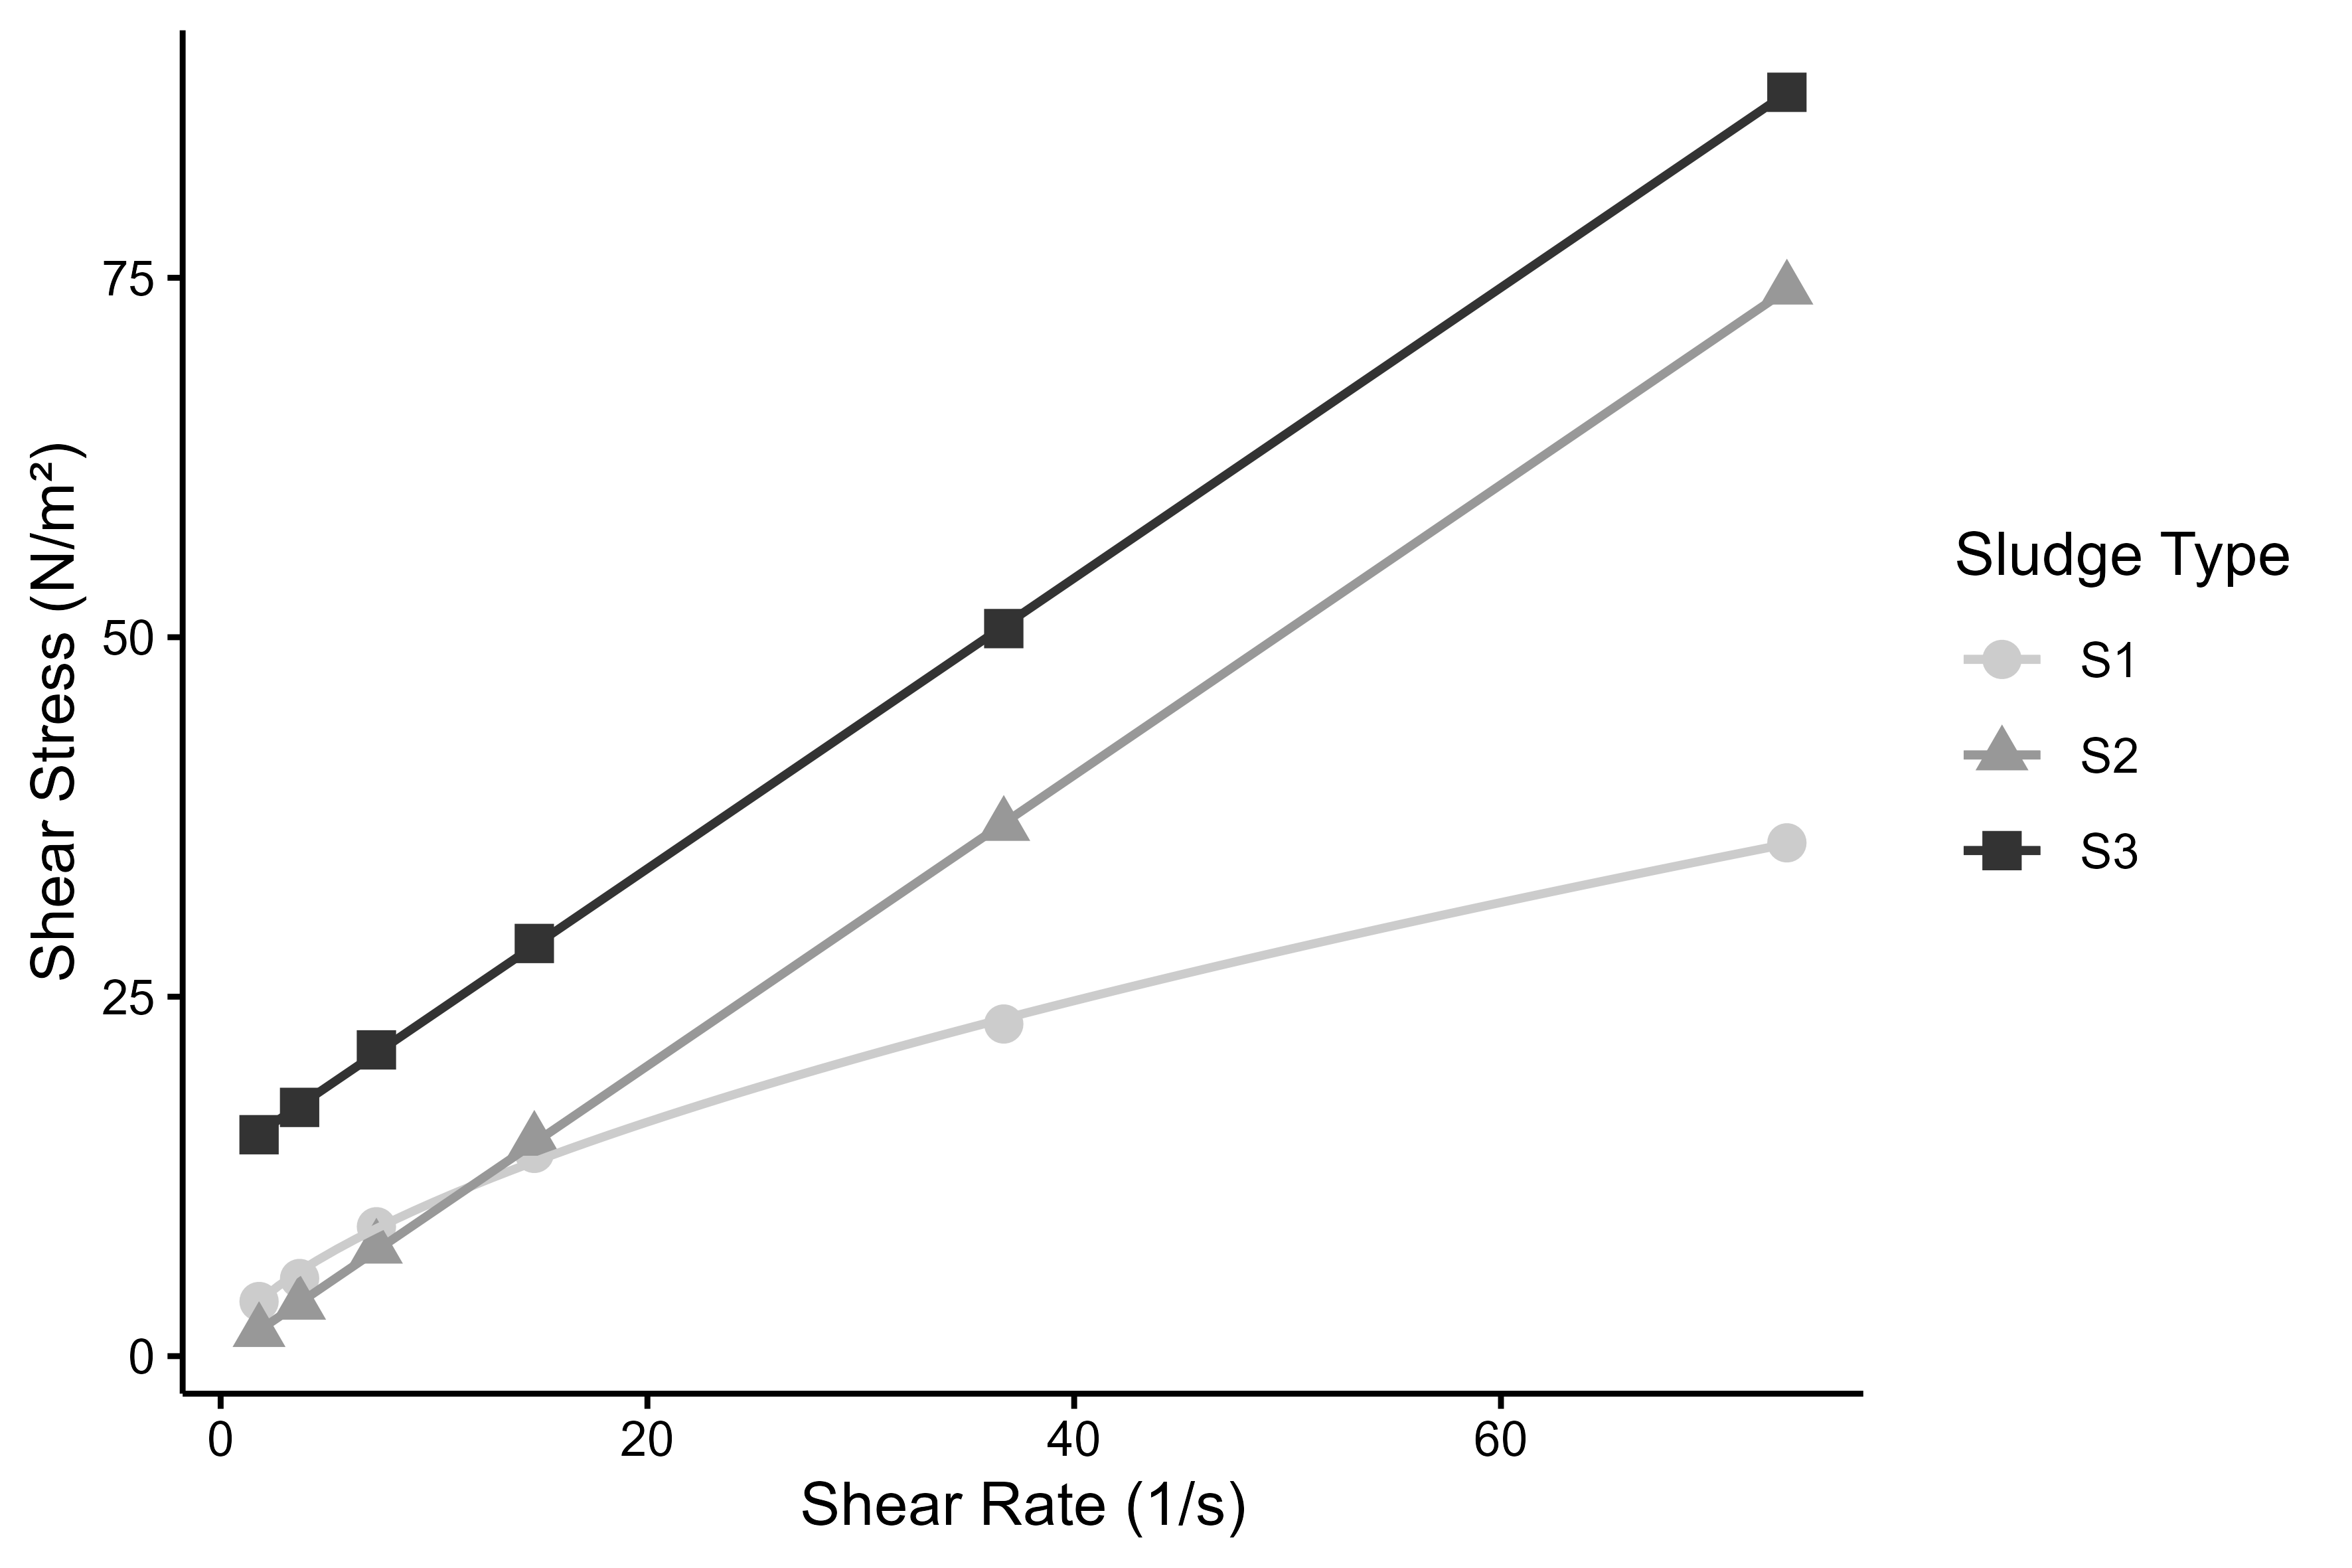
\includegraphics[scale=1]{homeworks/hw2/sludgeShear.png}
    \caption{Sludge rheology for 3 types of sludges}
    \label{fig:SludgeShear}
\end{figure}
\section{}
\cite{sanin2011}\todo{Q4 - Check the reference for table Hazen-Williams Coefficients for Various Solids Concentrations of Raw Sludge}\todo{Q4 - Is Hazen-Williams right? Is there another solution?}
\begin{minipage}[c]{0.6\textwidth}
FORMULAS
\end{minipage}
\hfill
\begin{minipage}{0.3\textwidth}
\fbox{\parbox{0.95\textwidth}{\textbf{Assumptions}\\Full pipe, pressurized flow\\No exit or minor losses\\EQN???}}
\end{minipage}
\printbibliography
\end{document}